\RequirePackage{luatex85,shellesc}
\documentclass[crop,tikz]{standalone}
\usepackage{pgfplots}
\usetikzlibrary{patterns, intersections, calc}
\begin{document}

\newcommand\TableWithBeaker[3]{
    \begin{scope}
        \coordinate (left) at ($#1-(#2/2,0)$);
        \path[top color=black, draw=none]  (left) rectangle ($#1+(#2/2,-0.2)$);
        \draw[very thick, red] (left) -- ($#1+(#2/2-0.1,0)$) -- ++(0,#3);
        \draw[very thick, red] (left) -- ++(0,#3);
    \end{scope}
}

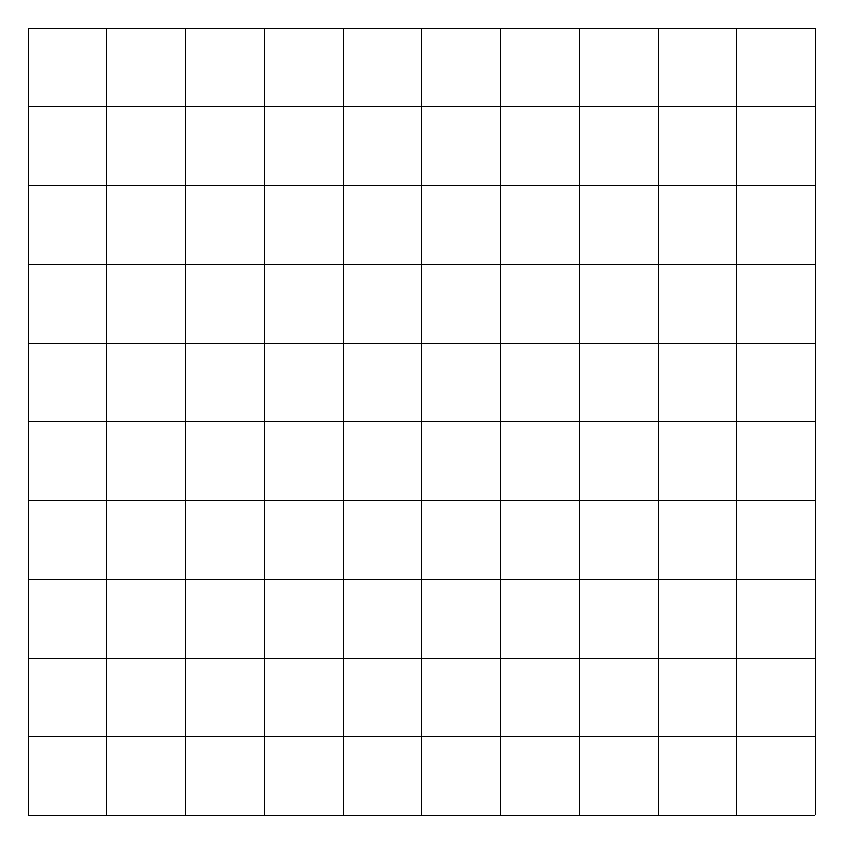
\begin{tikzpicture}[scale=1 , every node/.style={} ]
    % draw vibrating table.
    \draw[very thin] (-5,-5) grid (5,5);

    \TableWithBeaker{(0,0)}{4}{2};
    
\end{tikzpicture}	

\end{document}

